\chapter{L'optique physique}
\label{sec:op-detail}

% \section*{Rappels d'analyse vectorielle}
% Soient un vecteur $P$ et un réel $\lambda$. Rappelons que 
% \begin{equation}
% \label{eq:div_scal}
% \nabla\cdot(\lambda P) = P\cdot\nabla\lambda\ + \lambda\nabla\cdot P.
% \end{equation}


% Rappelons aussi la relation bien connue :
% \begin{equation}
% \label{eq:vect_id}
% \nabla\times\nabla\times P = \nabla\left(\nabla\cdot P\right)-\nabla^2P.
% \end{equation}

% Rappelons également qu'en coordonnées sphériques, le laplacien $\nabla^2$ s'écrit :
% \begin{equation}
% \nabla^2 = \inv{r^2}\derpart{}{r}\left(r^2\derpart{}{r}\right)+\inv{r^2\sin\theta}\derpart{}{\theta}\left(\sin\theta\derpart{}{\theta}\right)+\inv{r^2\sin^2\theta}\derderpart{}{\phi}.
% \end{equation}

% \'Etant donné un vecteur unitaire $n$ normal au vecteur $P$, on remarque que :
% \begin{equation}
% 	\label{eq:vect_normale}
% 	n\times P\times n = P.
% \end{equation}

% En effet :
% \begin{align*}
% 	n\times P\times n & = \left(\begin{array}{c}
% 		 n_1 \\
% 		 n_2 \\
% 		 n_3
% 	\end{array} \right) \times 
% 	\left(\begin{array}{c}
% 		 P_1 \\
% 		 P_2 \\
% 		 P_3
% 	\end{array} \right) \times 
% 	\left(\begin{array}{c}
% 		 n_1 \\
% 		 n_2 \\
% 		 n_3
% 	\end{array} \right) \\
% 	& = \left(\begin{array}{c}
% 		 n_2\left(P_1n_2-P_2n_1\right)-n_3\left(P_3n_1-P_1n_3\right) \\
% 		 n_3\left(P_2n_3-P_3n_2\right)-n_1\left(P_1n_2-P_2n_1\right) \\
% 		 n_1\left(P_3n_1-P_1n_3\right)-n_2\left(P_2n_3-P_3n_2\right)
% 	\end{array} \right)\\
% 	& = \left(\begin{array}{c}
% 		 \left(n_2^2+n_3^2\right)P_1-n_1\left(n_2P_2+n_3P_3\right)\\
% 		 \left(n_1^2+n_3^2\right)P_2-n_2\left(n_1P_1+n_3P_3\right)\\
% 		 \left(n_1^2+n_2^2\right)P_3-n_3\left(n_1P_1+n_2P_2\right)
% 	\end{array} \right)\\
% 	& = \left(\begin{array}{c}
% 		 \left(n_1^2+n_2^2+n_3^2\right)P_1-n_1\left(n_1P_1+n_2P_2+n_3P_3\right)\\
% 		 \left(n_1^2+n_2^2+n_3^2\right)P_2-n_2\left(n_1P_1+n_2P_2+n_3P_3\right)\\
% 		 \left(n_1^2+n_2^2+n_3^2\right)P_3-n_3\left(n_1P_1+n_2P_2+n_3P_3\right)
% 	\end{array} \right)\\
% 	& = \left(\begin{array}{c}
% 		  ||n||^2P_1+n_1(n\cdot P)\\
% 		  ||n||^2P_2+n_2(n\cdot P)\\
% 		  ||n||^2P_3+n_3(n\cdot P)
% 	\end{array} \right) = 
% 	    \left(\begin{array}{c}
% 		  P_1\\
% 		  P_2\\
% 		  P_3		 
% 	\end{array} \right) = P\\
% \end{align*}


\section{L'équation de radiation}
\label{seq:eqrad}
	\subsection{Solution pour une distribution quelconque de sources}
		\subsubsection{Solution générale de radiation en fonction de la distribution de sources}
On rappelle les équations de Maxwell:
\begin{subequations}
	\begin{equation}
		\nabla \cdot{} D = \rho, \label{eq:divD}
	\end{equation}

	\begin{equation}
		\nabla \cdot B = 0, \label{eq:divB} 
	\end{equation}

	\begin{equation}
		\nabla \times E = - \derpartt{B}, \label{eq:rotE}
	\end{equation}

	\begin{equation}
		\nabla \times H = J + \derpartt{D}, \label{eq:rotH}
	\end{equation}
	
	auxquelles on adjoint une équation de continuité :
	\begin{equation}
		\label{eq:cont}
		\nabla\cdot\J + \derpartt{\rho} = 0,
	\end{equation}
\end{subequations}
%
où l'on a posé $D = \epsilon_0 E$ et $H = B/\mu_0$, et avec $\epsilon_0$ la permittivité diélectrique du matériau, $\mu_0$ sa perméabilité magnétique $\rho$ la densité volumique de charges électriques et $J$ la densité volumique de charges électrique.

En prenant le rotationnel de l'équation (\ref{eq:rotE}), on obtient 
\begin{equation}
	\nabla\times\nabla\times E = -\derpartt{}(\nabla\times B),
	\label{eq:rotrotE}
\end{equation}
%
car les opérateur différentiels sont commutatifs si les champs sont suffisamment réguliers. En réinjectant (\ref{eq:rotH}) dans (\ref{eq:rotrotE}), on obtient :

\begin{equation}
	\label{eq:radtmp}
	\nabla\times\nabla\times E = -\mu_0\derpartt{J} -\mu_0\epsilon_0 \derderpartt{E}.
\end{equation}

Si le champ électrique est de la forme $E = \mathbf{E}e^{j\omega t}$,  et que l'on pose $k = \omega\sqrt{\mu_0\epsilon_0}$, alors l'équation (\ref{eq:radtmp}) se réécrit comme l'équation dite "Helmoltz vectorielle" :
\begin{subequations}
	\begin{equation}
		\label{eq:helmoltz}
		\nabla\times\nabla\times \mathbf E -k^2 \mathbf E = -j\omega\mu_0\mathbf J.
	\end{equation}
	De même, l'équation de continuité \eqref{eq:cont} se réécrit :
	\begin{equation}
		\label{eq:cont2}
		\nabla\cdot\J +j\omega\rho = 0.
	\end{equation}
\end{subequations}

On intègre maintenant ces équations grâce au théorème de Green vectoriel.
\begin{theorem}
	\label{th:green}
	\'Etant donné un volume $V$ borné par les surfaces $S_1,\dots,S_n$, soient $ F$ et $ G$ deux
	 vecteurs dépendant de la position dans la région et C$^2$ dans $V$, et notons $\mathbf n$ le
	  vecteur normal à une surface frontière orienté vers l'intérieur de $V$ :
	\begin{multline}
		\label{eq:green}
		\int_V\left( F\cdot\nabla\times\nabla\times G -  G\cdot\nabla\times\nabla\times F\right)
		\textrm{d}\mathcal{V} \\= -\int_{S_1+\dots+S_n}\left(F\times\nabla\times G-G \times\nabla
		\times F\right)\cdot \mathbf n \textrm{d}\mathcal{S}.
	\end{multline}
\end{theorem}

Supposons qu'il existe un volume $V$ borné par les surfaces $S_1,\dots,S_n$ dans lequel les champs $\mathbf E$ et $\mathbf B$ sont suffisamment réguliers. Soit un point $P$ dans le volume $V$. On définit la fonction $G$ :
\begin{equation}
	\label{eq:greenG}
	G = \frac{e^{-jkr}}{r}\mathbf{a} = \psi \mathbf{a},
\end{equation}
%
où $r$ est la distance de $P$ à un tout autre point de $V$ est $\mathbf{a}$ est un vecteur arbitraire constant.

La fonction $G$ vérifie les conditions de régularité du théorème de Green, sauf au voisinage de $P$ où elle est singulière. Soit donc une sphère $\Sigma$ de centre $P$ et de rayon $r_0$, et considérons $V'$ la région de $V$ borné par $S_1,\dots,S_n,$ et $\Sigma$ (que nous noterons dans la suite $\Gamma$ par simplicité).

On peut appliquer le théorème \ref{th:green} en prenant $F = \mathbf E$. L'équation \eqref{eq:green} devient alors :
\begin{multline}
	\label{eq:green_app}
	\int_{V'}\left( \psia\cdot\nabla\times\nabla\times \E -  \E\cdot\nabla\times\nabla\times \psia
	\right)\textrm{d}\mathcal{V} \\= -\int_\Gamma\left(\psia\times\nabla\times \E-\E \times\nabla
	\times \psia\right)\cdot \mathbf n \textrm{d}\mathcal{S}.
\end{multline}

On démontre très simplement à l'aide des relations (\ref{eq:div_scal}) et (\ref{eq:vect_id}) que 
\begin{equation}
	\label{eq:helm_green_app}
	\helm\psia = \nabla(\mathbf{a}\cdot\nabla\psi)+k^2\psia.
\end{equation}

\`A partir des équations \eqref{eq:helmoltz} et \eqref{eq:helm_green_app}, on obtient :
\begin{equation}
	\label{eq:tmp1}
	\psia\cdot\helm\E-\E\cdot\psia
	= -j\omega\mu_0\psia\cdot\J-\E\cdot\nabla(\mathbf a\cdot\nabla\psi).
\end{equation}
%
En remarquant en plus qu'avec l'équation \eqref{eq:divD} l'on obtient 
\begin{equation}
	\label{eq:tmp2}
	\begin{array}{rl}
		\E\cdot\nabla(\mathbf a\cdot\nabla\psi) &= \nabla\cdot[\E(\mathbf a\cdot\nabla\psi)] -
		 (\mathbf a\cdot\nabla\psi)\nabla\cdot\E\\
		&=\nabla\cdot[\E(\mathbf{a}\cdot\nabla\psi)] - \dfrac{\rho}{\epsilon}\mathbf a\cdot\nabla
		\psi,
	\end{array}
\end{equation}
%
l'équation \eqref{eq:green_app} prend alors la forme suivante
\begin{multline}
	\label{eq:tmp3}
	\mathbf a \cdot\int_{V'}\left(j\omega\mu_0\psi\J-\frac{\rho}{\epsilon_0}\nabla\psi\right)\di{V} 
	+ \int_{V'}\nabla\cdot[\E(\mathbf{a}\cdot\nabla\psi)]\di{V} \\
	= \int_\Gamma \left[(\E\times\nabla\times\psia)\cdot\mathbf n-(\psia\times\nabla\times\E)\cdot
	\mathbf{n}\right]\di{S}.
\end{multline}

La seconde intégrale de volume peut être exprimée comme une intégrale de surface :
\begin{equation}
	\int_{V'}\nabla\cdot[\E(\mathbf a\cdot\nabla\psi)]\di V = - \int_\Gamma \E(\mathbf a\cdot\nabla
	\psi)\cdot\mathbf n\di S = - \mathbf{a} \cdot\int_\Gamma (\E\cdot\nabla\psi)\cdot\mathbf n\di S 
	.
\end{equation}
%
De plus, remarquons que :
\begin{equation}
	[\E\times(\nabla\times\psia)]\cdot\mathbf n = [\E\times\nabla\psi\times\mathbf a)]\cdot\mathbf 
	n = [(\mathbf n\times\E)\times\nabla\psi]\cdot\mathbf a.
\end{equation}
%
Enfin, en utilisant \eqref{eq:rotE}, on montre que :
\begin{equation}
	\psi(\mathbf a\times\nabla\times\E)\cdot\mathbf n = j\omega\psia\cdot(\mathbf n\times\B).
\end{equation}

Appliquer ces trois transformations dans l'équation \eqref{eq:tmp3} permet d'exprimer chaque membre comme un produit scalaire entre $\mathbf{a}$ et une intégrale. Comme cette équation doit être vérifiée quelque soit $\mathbf a$, cela implique l'égalité entre les intégrales elles-mêmes. En séparant l'intégrale sur $\Sigma$ des autres intégrales de surface, par commodité pour la suite, cela donne :
\begin{multline}
	\label{eq:oof}
	\int_\Sigma[-j\omega\psi(\mathbf n\times\B)+(\mathbf n \times \E)\times\nabla\psi+(\mathbf n
	\cdot\E)\nabla\psi]\di S =
	\\ \int_{V'}\left(j\omega\psi\mu_0\J - \frac{\rho}{\epsilon_0}\nabla\psi\right)\di V 
	\\- \int_{S_1+\dots+S_n}[-j\omega\psi(\mathbf n\times\B)+(\mathbf n \times \E)\times\nabla\psi+
	(\mathbf n\cdot\E)\nabla\psi]\di S.
\end{multline}

Considérons maintenant l'intégrale sur la surface $\Sigma$. On a 
\begin{equation}
	\nabla\psi = \left[\derr{}\left(\frac{e^{-jkr}}{r}\right)\right]_{r=r_0}\mathbf n = -\left(jk+
	\inv{r_0}\right)\frac{e^{-jkr_0}}{r_0}\mathbf n.
\end{equation}

L'intégrale peut alors être écrite :
\begin{equation}
	\int_\Sigma[\ ]\di S = -4\pi jr_0e^{-jkr_0}\left(\omega\overline{\mathbf{n}\times \B}+k
	\overline{\E}\right)-4\pi e^{-jkr_0}\overline{\E},
\end{equation}
%
où la barre superieure représente la valeur de la fonction moyennée sur la surface $\Sigma$. Par hypothèse, le champ $\B$ est fini au voisinage de $P$, donc si l'on fait tendre $r_0$ vers 0, le premier terme du second membre disparaît. Dans le même temps, la valeur de $\overline{\E}$ tend vers $\E_P$, la valeur du champ électrique en $P$. Ainsi :

\begin{equation}
	\lim_{r_0\to0}\int_\Sigma[\ ]\di S = -4\pi\E_P.
\end{equation}

De plus, dans cette hypothèse, la région $V'$ en vient à être égale à $V$. L'équation \eqref{eq:oof} devient alors

\begin{multline}
	\label{eq:general_solution}
	\E_P = -\inv{4\pi} \int_{V}\left(j\omega\psi\mu_0\J - \frac{\rho}{\epsilon_0}\nabla\psi\right)
	\di V 
	\\+ \inv{4\pi} \int_{S_1+\dots+S_n}[-j\omega\psi(\mathbf n\times\B)+(\mathbf n \times \E)\times
	\nabla\psi+(\mathbf n\cdot\E)\nabla\psi]\di S.
\end{multline}

		\subsubsection{Solution de l'équation de radiation pour un domaine non borné}
		\label{sec:unbound}
On se place maintenant dans le cas particulier où le volume $V$ n'est pas borné, mais que la distribution de sources est confinée dans une région bornée. Soit donc une sphère $S(R)$ de centre $P$ et de rayon $R$ suffisamment grand pour que toutes les sources soient incluses dans la sphère. Soit aussi un champ de vecteurs unitaires $\R_1$ colinéaire au rayon de la sphère et dirigé vers l'extérieur. On note $\mathbf n = -\R_1$.  En notant $\psi$ sous sa forme explicité, l'intégrale surfacique de l'équation \eqref{eq:general_solution} s'écrit alors : 
\begin{multline}
	\inv{4\pi} \int_S[-j\omega\psi(\mathbf n\times\B)+(\mathbf n \times \E)\times\nabla\psi
	+(\mathbf n\cdot\E)\nabla\psi]\di S 
	\\= \inv{4\pi} \int_S \left\{j\omega\left[(\R_1\times\B)+\sqrt{\mu_0\epsilon_0}\E\right]
	+\frac{\E}{R}\right\}\frac{e^{-jkR}}{R} \di S.
\end{multline}

Cette intégrale de surface disparaît lorsque  $R\to+\infty$ si le champs $\E$ satisfait les conditions suivantes :
\begin{subequations}
	\label{eq:hypo}
	\begin{equation}
		\label{eq:hypo_finite}
		\lim_{R\to\infty} R\E \text{ is finite,}
	\end{equation}
	\begin{equation}
		\label{eq:hypo_nulle}
		\lim_{R\to\infty} R\left[(\R_1\times\B)+\sqrt{\mu_0\epsilon_0}\E\right] = 0.
	\end{equation}
\end{subequations}

Si le champ électrique satisfait ces conditions, alors :

\begin{equation}
	\E_P = -\inv{4\pi} \int_{V}\left[j\omega\mu_0\J\frac{e^{-jkr}}{r} - \frac{\rho}{\epsilon_0}\nabla
	\left(\frac{e^{-jkr}}{r}\right)\right]\di V.
\end{equation}

\'A l'aide de l'équation de continuité \eqref{eq:cont2}, on peut exprimer le second membre de l'équation précédente uniquement en termes de densité de courant:

\begin{equation}
	\E_P = \frac j{4\pi\omega\epsilon_0} \int_{V}\left[-k^2\J\frac{e^{-jkr}}{r} 
 + (\nabla\cdot\J)\nabla\left(\frac{e^{-jkr}}{r}\right)\right]\di V.
\end{equation}

Enfin, si $R$ est suffisamment grand pour que toutes les distributions de courants soient contenues à l'intérieur de $S$, alors on peut montrer que :

\begin{equation}
	\label{eq:unbound}
	\E_P = -\frac j{4\pi\omega\epsilon_0} \int_{V}\left[k^2\J 
	+ (\J\cdot\nabla)\nabla\right]\frac{e^{-jkr}}{r}\di V.
\end{equation}

\paragraph{N.B.:} Il est important de se souvenir que l'équation \eqref{eq:unbound} n'est valable que sous réserve que les hypothèses \eqref{eq:hypo} soient vérifiée !

		\subsubsection{Solution champ lointain}
		\label{sec:champloin}
En section \ref{sec:unbound}, on a supposé que les sources sont confinées dans une région finie de l'espace. Choisissons donc une origine $O$ au voisinage de cette région. Soit un point $P$ dans $V$. Notons $\R_S$ le vecteur de l'origine à l'élément de source $S$ situé au point $(x,y,z)$, $R\R_1 = \vect{OP}$ et $r\rr_1 = \vect{SP}$, $\R_1$ et $\rr_1$ étant des vecteurs unitaires. On traite le point $P$ comme une origine fixe. Ainsi, l'opérateur $\nabla$ n'agit que sur les coordonnées du point source. Ainsi, l'intégrande de l'équation \eqref{eq:unbound} s'écrit uniquement en une somme de puissances de $r^{-1}$. En se restreignant aux termes de premier ordre, on a :
\begin{equation}
	\label{eq:firstorder}
	 -\frac j{4\pi\omega\epsilon_0} \int_{V} \left[k^2\J - k^2(\J\cdot\rr_1)\rr_1\right]
	\frac{e^{-jkr}}{r}\di V.
\end{equation}

On se place dans le cas où $P$ est très éloigné du point source le plus éloigné de l'origine ($R >> ||\R_S||$). Ainsi, $\rr_1$ et $\R_1$ peuvent être considérés comme colinéaires et l'un remplacé par l'autre. De même, $r^{-1}\approx R^{-1}$ au premier ordre en $R^{-1}$. Enfin, on peut écrire  :

\begin{equation}
	r = R-\R_S\cdot\R_1.
\end{equation}

Avec ces approximations, et en gardant bien en tête que $R$ est une constante, l'équation \eqref{eq:unbound} se réécrit :

\begin{equation}
	\label{eq:far_field}
	\E_P = -\frac{j\omega\mu_0}{4\pi R}e^{-jkR}\int_V\left[\J-(\J\cdot\R_1)\R_1\right]
	e^{jk\R_S\cdot\R_1}\di V + \mathcal O\left(\inv{R^2}\right).
\end{equation}

Remarquons que l'intégrale du second membre de \eqref{eq:far_field} ne dépend pas de $r$. L'équation \eqref{eq:hypo_finite} est donc vérifiée. De plus, un rapide calcul, laissé en exercice pour le lecteur, montre que \eqref{eq:hypo_nulle} est également vérifiée dans cette approximation. 

Enfin le produit scalaire entre \eqref{eq:hypo_nulle} et $\R_1$ permet de montrer que le champ $\E$ est perpendiculaire à la fois à $\B$ et à $\R_1$ (au premier ordre en $R$). On peut donc approximer le champ EM lointain à une onde plane.

Afin de simplifier une dernière fois l'équation, introduisons au point $P$ un système de coordonnées polaires $\left(\er,\et,\ep\right)$, avec $\er = \R_1$. On décompose le champ électrique ainsi : $$\E_P = \E_r+\E_\theta+\E_\phi = (\E_P\cdot\er)\er + (\E_P\cdot\et)\et +(\E_P\cdot\ep)\ep$$Comme on vient de le dire, on a $$\E_r = \vect 0.$$ Dans ce système de coordonnées, les deux composantes non nulles du champ électrique s'écrivent :
\begin{subequations}
	\begin{align}
			\E_\theta &= -\frac{j\omega\mu_0}{4\pi R}e^{-jkR}\int_V\left(\J\cdot\et\right)
				e^{jk\R_S\cdot\R_1}\di V \et\\
			\E_\phi &= -\frac{j\omega\mu_0}{4\pi R}e^{-jkR}\int_V\left(\J\cdot\ep\right)
				e^{jk\R_S\cdot\R_1}\di V \ep
	\end{align}
\end{subequations}



	\subsection{Puissance transmise}
	
Vecteur de Poynting (approx champ lointain $\to$ onde plane):
\begin{equation}
	S = \inv{2\mu_0} \Re(\E\times\B^*) = \inv{2Z_0}\left(|\E_\theta|^2+|\E_\phi|^2\right)\R_1
\end{equation}

Puissance rayonnée par unité d'angle solide :
\begin{equation}
	P(\theta,\phi) = R^2|S| = \frac{R^2}{2Z_0}\left(|\E_\theta|^2+|\E_\phi|^2\right)
\end{equation}

\section[Courant électrique]{Calcul du champ de densité de courant électrique}
	\subsection{Condition de saut à travers une fine plaque conductrice}

Considérons une plaque plane présentant une densité volumique de courant $\vect j$, de dimensions infines dans les directions $\ex$ et $\ey$ et s'étendant de $z = -a/2$ à $z = a/2$. Le reste de l'espace est vide ($\rho = 0$ et $\vect j = \vec0$). On note 1 le demi espace $z > a/ 2$ et 2 le demi espace $z > a/2$. Cette plaque est éclairée depuis le demi-espace 2 par un champ électromagnétique $(\E,\B)$.

On pose $$\vect{j_S} = \int_{-\frac a2}^{\frac{a}{2}}\vect j\dd z.$$

Les directions $\ex$ et $\ey$, ainsi que l'évolution temporelle, ne sont pas influencées par la géométrie du système. Ainsi on peut considérer que, pour $i = {x,y,z}$ :
\begin{equation}
	\label{eq:saut_hypo}
	\int_{-\frac a2}^{\frac{a}{2}} \derpartx{E_i}  \dd z \approx 0; \ 
	\int_{-\frac a2}^{\frac{a}{2}} \derpart{E_i}{y}\dd z \approx 0; \ 
	\int_{-\frac a2}^{\frac{a}{2}} \derpartt{E_i}  \dd z \approx 0. \ 
\end{equation}

L'intégration de la seconde équation de Maxwell \eqref{eq:divB} combinée à l'hypothèse \eqref{eq:saut_hypo} permet de montrer que :
\begin{equation}
	\label{eq:saut_z}
	B_{z,2} = B_{z,1}.
\end{equation}

Similairement, on montre en intégrant la quatrième équation de Maxwell \eqref{eq:rotH} et en utilisant les hypothèses \eqref{eq:saut_hypo} que :
\begin{equation}
	\label{eq:saut_autres}
	\left\{\begin{array}{l}
	-\left(B_{y,2} - B_{y,1}\right) = \mu_0j_{S_x} \\
	B_{x,2} - B_{x,1} = \mu_0j_{S_y} \\
	j_{S_z} = 0
	\end{array} \right.
\end{equation}

Si on l'on note $\vect{n_{12}}$ la normale à la surface de la plaque orientée en direction des $z \nearrow$, on peut réécrire l'équation précédente ainsi :
\begin{equation}
	\label{eq:saut_vect}
	\vect{B_2}-\vect{B_1} = \mu_0 \vect j_s\times\vect{n_{12}}.
\end{equation}

En pratique, dans les cas d'une plaque conductrice très fine, où $a \to 0$, la densité volumique de courant devient très importante, ce qui fait que $\vect{j_S}$ et donc les seconds membres de \eqref{eq:saut_autres} conservent des valeurs non négligeables même pour des valeur de $a$ très faibles. En fait, on montre très facilement que dès que $a$ et la courbure sont suffisamment faibles devant les dimensions du problème, l'équation \eqref{eq:saut_vect} est la forme générale de la condition de saut.

	\subsection{Cas d'un matériau parfaitement conducteur}
	\label{sec:saut_pec}

D'après un résultat classique de l'électromagnétisme, lorsqu'un matériau parfaitement conducteur est éclairé par un champ électromagnétique, le champ magnétique est nul dans le matériau, et la distribution volumique de courant est en fait confinée à une surface infiniment fine à l'interface entre le matériau et le vide en une distribustion surfacique de courant $\vect{j_S}$. Dans ces conditions, on se ramène donc au cas précédent avec un $a$ très petit et $\vect{B_1} = \vect 0$.

L'équation \eqref{eq:saut_vect} devient alors :
\begin{equation}
	\vect{B_2} = \mu_0 \vect j_s\times\vect{n_{12}}.
\end{equation}

Puisque $\vect{j_S}$ est tangent à la surface et donc normal à $\vect{n_{12}}$, alors l'équation précédente combinée à \eqref{eq:vect_normale} permet de donner une valeur à $\vect{j_S}$ en fonction uniquement du champ magnétique incident :

\begin{equation}
	\label{eq:saut_courant}
	\vect{j_S} = \inv{\mu_0}\vect{n_{12}}\times\vect{B_2}.
\end{equation}




\section[SER]{L'équation d'antenne et la section équivalente radar}
\label{sec:rcs}

On se place dans un cadre monostatique. Soient $G$ le gain de l'antenne, $P_t$ la puissance émise, $P_r$ la puissance réfléchie vers l'antenne, $\lambda$ la longueur d'onde d'émission, et $R$ la distance de la cible. La surface équivalente radar (SER) s'écrit :

\begin{equation}
	\sigma =\frac{(4\pi)^3R^4}{\lambda^2} \frac{P_r}{GP_t}=\frac{(4\pi)^3R^4}{G\lambda^2} \frac{|\E_\theta^r|^2+|\E_\phi^r|^2}{|\E_\theta^t|^2+|\E_\phi^t|^2},
\end{equation}
%
où $E_X^r$ est le champ électrique reçu et $E_X^t$ est le champ électrique émis par l'antenne.



\begin{equation}
	\label{eq:rcs_lim}
	\sigma = \lim_{R\to\infty}4\pi R^2 \frac{|\E_s|^2}{|\E_i|^2}
\end{equation}

\section[Approximation PO]{L'approximation Optique Physique}
\label{sec:equation_OP}

Considérons un volume $V$ consitué d'un matériau conducteur. Soit l'origine $O$ de l'espace, située à proximité de (éventuellement dans) $V$. \'Etant donné un point de $V$, notons $\R_S$ le vecteur allant de l'origine à ce point.

Considérons maintenant un point $P$ situé suffisamment loin de V pour que l'approximation champ lointain soit valable, ainsi qu'un système de coordonnées sphériques $\left(\er,\et,\ep\right)$ en $P$. Notons $\vect{OP} = R\er$, et $\E_P$ le champ électrique au point $P$.


Le volume $V$ est éclairé par un champ électromagnétique $\left(\E_i,\B_i\right)$ de fréquence $f$ assimilé à une onde plane selon un vecteur d'onde $\vect{k_i} = -\dfrac{2\pi f}{c}\eri = -k\eri$ (avec $\eri$ un vecteur unitaire), ce qui induit une distribution volumique de courant $\J$. En en point $M$ quelconque, le champ $\E_i$ s'écrit ainsi : $$\E_i = (E_{i,\theta}\eti + E_{i,\phi}\epi)e^{-j\ki\cdot\vect{OM}},$$ où $\eti$ $\epi$ sont deux vecteurs unitaires tels que ($\eri,\eti, \epi$) soit une base orthonormée directe. De plus, pour simplifier, le champ électrique électrique incident est considéré comme d'amplitude unitaire : $$||\E_i||^2 = |E_{i,\theta}|^2 + |\E_{i,\phi}|^2 = 1.$$

Le résultat de la section \ref{sec:champloin} donne : 

\begin{equation}
	\E_P = -\frac{jkZ_0}{4\pi R}e^{-jkR}\iiint\limits_V \left(J^\theta\et + J^\phi\ep\right) e^{jk\R_S\cdot\er} \di V,
\end{equation}
%
où l'on a posé $Z_0 = \sqrt{\dfrac{\mu_0}{\epsilon_0}}$, $J^\theta = \J\cdot\et$ et $J^\phi = \J\cdot\ep$.

Faisons l'approximation que le matériau est parfaitement conucteur.La distribution $\J$ devient alors une distribution surfacique $\J_s$ répartie à la frontière du volume $V$. L'équation précédente devient donc : 
\begin{equation}
	\label{eq:surfacique}
	\E_P = -\frac{jkZ_0}{4\pi R}e^{-jkR}\iint\limits_S \left(J_s^\theta\et+J_s^\phi\right) e^{jk\R_S\cdot\er} \di S.
\end{equation}

Approchons maintenant cette surface par un maillage surfacique à $N$ facettes triangulaire. Dans le cadre de l'approximation de l'optique physique, on considère que chaque facette est indépendante des autres. Le champ en $P$ est donc la superposition de tous les champs rayonnées par chaque facette :
\begin{equation}
	\label{eq:maillage}
		\E_P = -\frac{jkZ_0}{4\pi R}e^{-jkR}\sum_{l=1}^N\iint\limits_{S_l} \left(J_{s_l}^\theta\et + J_{s_l}^\phi\ep\right) e^{jk\R_S\cdot\er} \di S.
\end{equation}

Certaines de ces facettes sont dans l'ombre des autres. Dans le cadre de l'approximation de l'optique physique, on considère que la distribution de courant surfacique est nulle sur ces facettes. Pour les facettes éclairées, la distribution de courant surfacique est donnée par les résultats de la section \ref{sec:saut_pec} :

\begin{equation}
	\J_s = \left\{
	\begin{array}{cl}
		\dfrac{2}{\mu_0}\mathbf n\times\B_i & \text{dans la zone illuminée,}\\
		0 & \text{dans la zone d'ombre,}
	\end{array}\right.
\end{equation}
%
avec $\mathbf{n}$ la normale à la facette. Les détails de l'agorithme de faces cachées sont donnés dans la section \ref{sec:facescachees}.

Puisque le champ magnétique est une onde plane, on a :
\begin{equation}
	\B_i = \frac{\mu_0}{Z_0}\vect{k_i}\times\E_i = \frac{\mu_0}{Z_0}\left(E_{i,\phi}\eti-E_{i,\theta}\epi\right)e^{-j\R_s\cdot\ki}.
\end{equation}

La distribution de courants s'écrit donc :
\begin{equation}
	\J_s = \left\{
	\begin{array}{cl}
		\dfrac{2}{Z_0}\left(E_{i,\phi}\mathbf{n}\times\eti-E_{i,\theta}\mathbf{n}\times\epi
		\right)e^{-j\R_s\cdot\ki}. & \text{dans la zone illuminée,}\\
		0 & \text{dans la zone d'ombre.}
	\end{array}\right.
\end{equation}

Dans le cas général, le champ rayonné en $P$ s'écrit donc :
\begin{equation}
	\label{eq:rayon_bistat}
	\boxed{
	\E_P = - \frac{2jk}{4\pi R}e^{-jkR}\sum_{l=1}^N\left[\delta_l\left(J_{S_l}^\theta\et+J_{S_l}^\phi\ep\right)\iint\limits_{S_l}e^{j\R_s\cdot(k\er-\vect{k_i})}\di S\right],
	}
\end{equation}
%
où $\delta_l = 1$ si la facette $l$ est illuminée, et 0 si elle est cachée et avec :
\begin{align*}
	J_{S_l}^\theta &= \left(E_{i,\phi}\mathbf n_l\times\eti-E_{i,\theta}\mathbf n_l\times\epi\right)\cdot\et,
	\\ &\text{    et} \\
	J_{S_l}^\phi &= \left(E_{i,\phi}\mathbf n_l\times\eti-E_{i,\theta}\mathbf n_l \times\epi\right)\cdot\ep.
\end{align*}

Dans le cas particulier d'une observation monostatique, l'équation \eqref{eq:rayon_bistat} se simplifie un peu. En effet, dans ce cas, $\ki = -k\eri=-k\er$,$\eti = \et$ et $\epi = \ep$.

Notons en particulier que $$(\mathbf{n}\times\et)\cdot\ep = \mathbf n\cdot(\et\times\ep) = \mathbf n\cdot\er$$ et, similairement, $$(\mathbf{n}\times\ep)\cdot\et = \mathbf n \cdot(\ep\times\et) = -\mathbf n\cdot\er.$$

Ainsi, si l'on note $n_{l,r} = \mathbf n_l\cdot\er$, l'équation \eqref{eq:rayon_bistat} devient :
\begin{equation}
	\label{eq:rayon_monostat}
	\boxed{
	\E_P = - \frac{2jk}{4\pi R}e^{-jkR}\sum_{l=1}^N\left[\delta_l\left(E_{i,\theta}n_{l,r}\et+E_{i,\phi}n_{l,r}\ep\right)\iint\limits_{S_l}e^{2jk\R_s\cdot\er}\di S\right].
	}
\end{equation}

Pour la suite, on se place dans le cadre monostatique. Si l'on injecte l'équation \eqref{eq:rayon_monostat} dans la définition de la SER \eqref{eq:rcs_lim} donnée à la section \ref{sec:rcs}, on obtient :

\begin{equation}
	\sigma = \lim_{R\to\infty} \frac{k^2}{\pi||\E_i||^2} \left|\left|\sum_{l=1}^N\left[\delta_l\left(E_{i,\theta}n_{l,r}\et+E_{i,\phi}n_{l,r}\ep\right)\iint\limits_{S_l}e^{2jk\R_s\cdot\er}\di S\right]\right|\right|^2.
\end{equation}

L'expression dont on prend la limite ne dépendant pas de $R$, cela donne simplement :

\begin{equation}
	\label{eq:rcs}
	\boxed{\boxed{
	\sigma = \frac{k^2}{\pi} \left|\left|\sum\limits_{l=1}^N\left[\delta_l\left(E_{i,\theta}n_{l,r}\et+E_{i,\phi}n_{l,r}\ep\right)\iint\limits_{S_l}e^{2jk\R_s\cdot\er}\di S\right]\right|\right|^2.}}
\end{equation}

Intéressons nous à la valeur de l'intégrale de surface :
\begin{equation}
	\label{eq:integrale_osci}
	I = \int_\Sigma e^{2jk\vect r\cdot\er}\di S.
\end{equation}
Soit une surface plane triangulaire $\Sigma$, de sommets $P_1,P_2,P_3$ et de normale $\vect n$. Notons $P_0$ le barycentre de la facette. Pour $m\in\{0,1,2,3\}$ notons $\vect{r_m} = \vect{OP_m}$. Enfin notons respectivment $\vect{a_1},\vect{a_2},\vect{a_3} = \vect{P_1P_2},\vect{P_2P_3},\vect{P_3P_1}$.

Développons le produit scalaire $\R\cdot\er$ au premier ordre :
\begin{equation}
	\label{eq:gordon_dvp}
	\vect r\cdot\er\approx \vect{r_0}\cdot\er+\left(\vect r-\vect{r_0}\right)\cdot\vect{l_r},
\end{equation}
%
où l'on a posé (dans le cas monodimensionel):
\begin{equation}
	\label{eq:gordon_lr}
	\vect{l_r} = -2\er
\end{equation}

Posons $Q = |\vect n\times\vect{l_r}|$ et $\vect q = \dfrac{\vect n\times\vect{l_r}}{Q}$.

La formule de Gordon donne :

\begin{equation}
	\label{eq:gordon_res}
	\boxed{
	I = \frac{j}{2kQ}\sum_{m=1}^3\left(\epsilon_m\vect q\cdot\vect{a_m}\right)e^{-2jk\left(\vect{r_m}-\vect{r_0}\right)\cdot\vect{l_r}}\sinc\left(\frac{2k\vect{l_r}\cdot\vect{a_m}}{2}\right).
	}
\end{equation}

Avec $\epsilon_m = 0$ si la barre numéro $m$ est à la frontière entre une facette éclairée et une facette cachée et n'est pas une arête franche, et $\epsilon_m = 1$ sinon. Ce terme est ajouté pour limiter la diffraction parasite à la discontinuité entre zone d'ombre et zone éclairée. % (\`A SOURCER).

Dans le cas $Q \to 0$, l'équation précédente est équivalente à :
\begin{equation}
	\label{eq:gordon_res_0}
	%I = Se^{jk\vect{r_0}\cdot\vect{l_r}}
	I = S
\end{equation}


\section{PTD}
\label{sec:PTD}
Dans cette section, je présente succintement la théorie physique de la diffraction (PTD) proposée par Michaeli en 1986. Pour plus de détails, je vous renvoie à l'article original \cite{Michaeli1986a}.
% Pas encore implémentée

Le principe de cette méthode est d'ajouter un terme correctif $I^f$ à la densité de courant surfacique sur les arêtes. Ce terme dépend de la géométrie des deux facettes adjacentes à l'arête et du nombre d'onde $k$ : $$I^f = I_1^f - I_2^f$$ où $I_n^f$ est la contribution de l'arête $n$ au terme correctif de la diffraction.

\paragraph{}
Le terme correctif de l'arête 1 est donné par l'expression : 
\begin{equation}
	\begin{split}
		I_1^f =& -\frac{2j}{kZ_0\sin^2\beta}\left\{\frac{\sin\phi \delta(\pi-\theta)}{\cos\phi+\mu} + \frac{(1/N)\sin(\phi/N)}{\cos[(\pi-\alpha)/N] - \cos(\phi/N)}\right\} \mathbf z\cdot\E\inc  \\
		& + \frac{2j\sin[(\pi - \alpha)/N]}{Nk\sin\beta\sin\alpha}\frac{\mu\cot\beta'-\cot\beta\cot\phi}{\cos(\phi/N)-\cos[(\pi-\alpha)/N]}\mathbf z\cdot\Hh\inc
	\end{split}
\end{equation}
%
où $\delta(x) = 1$ si $x > 0$ et $\delta(x) = 0$ sinon, $\mu = \sin\beta\cos\phi/\sin\beta'$ et $\alpha = -j\ln(\mu + j\sqrt{1-\mu^2})$. Les angles $\beta$, $\beta'$ et $\phi$ et la quantité $N$ sont définies dans la figure \ref{fig:PTD}.

\begin{figure}[htp]
	\centering
	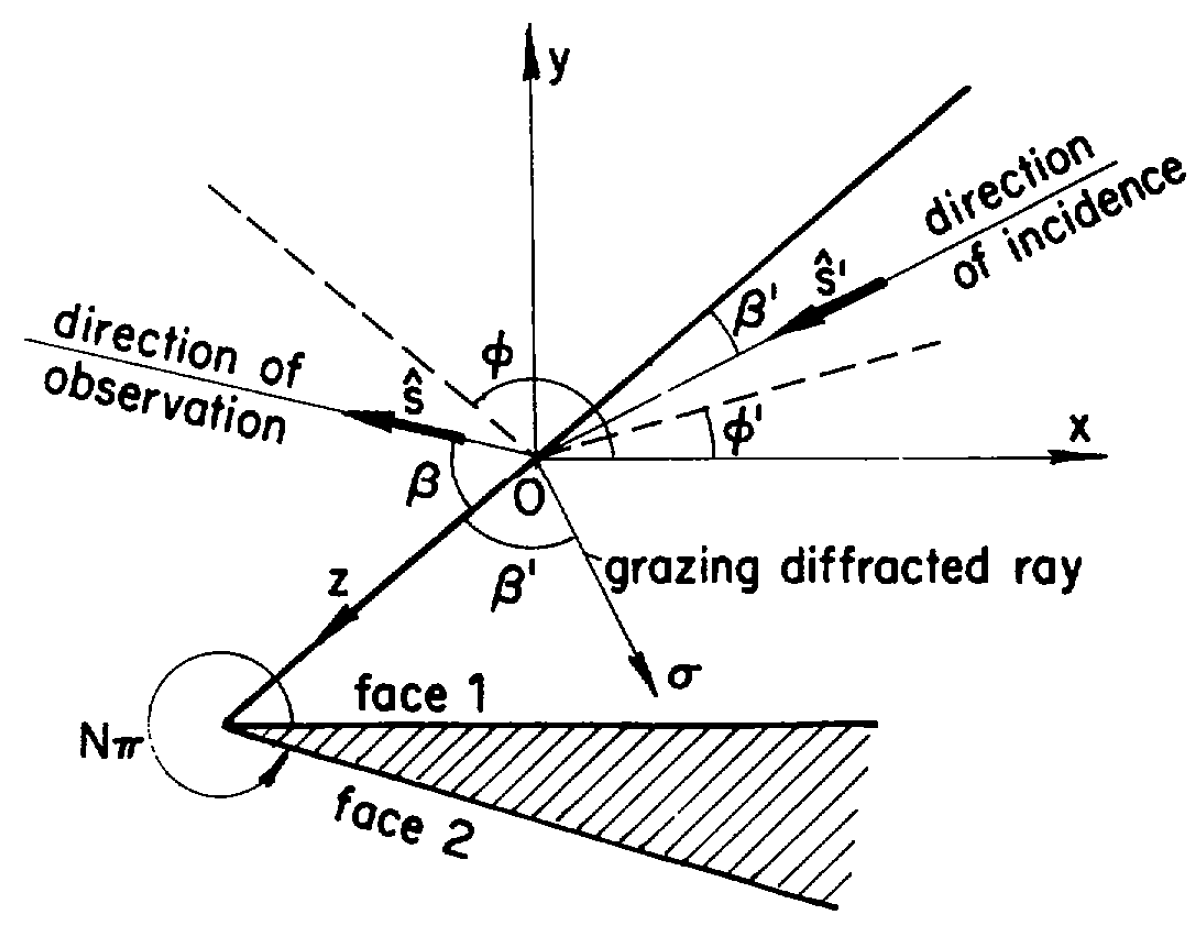
\includegraphics[width=0.75\textwidth]{images/PTD.png}
	\caption{Géométrie de la diffraction d'arête. Les lignes pointillées représentent les projections des directions d'incidence et d'observation sur le plan $xy$. Image tirée de \cite{Michaeli1986a} (figure 1).}
	\label{fig:PTD}
\end{figure}

\paragraph{}
L'expression du terme correctif de la facette 2 $I^f_2$ s'obtient à partir de $I^f_1$ en applicant les transformations suivantes :
\begin{equation}
	\begin{split}
		\mathbf z\to-\mathbf z,\quad \phi\to N\pi - \phi \\
		\beta\to\pi-\beta,\quad \beta'\to\pi-\beta'
	\end{split}
\end{equation}

\section{Description du code}
\label{sec:code}
\begin{enumerate}
	\item Lecture des cartes d'entrée
	\item Lecture du maillage
	\item Calcul des éléments voisins d'éléments
	\item Detection des arêtes %(voir section \ref{sec:aretes})
	\item Boucle sur les directions d'observations
	\begin{enumerate}
		\item Calcul de $\vect{l_r}$ (eq \eqref{eq:gordon_lr})
		\item Boucle sur les facettes
		\begin{enumerate}
			\item Calcul du barycentre de la facette
			\item Calcul de la normale à la facette
			\item Calcul de $S$, $\vect q$, et $Q$
			\item \'Elimination des barres frontières
			\item Calcul de $I$ par l'équation \eqref{eq:gordon_res} ou l'équation \eqref{eq:gordon_res_0}
		\end{enumerate}
		\item Boucle sur les arêtes
		\begin{enumerate}
			\item Identification des facettes adjacentes
			\item Calcul des angles $\beta$, $\beta'$, $\phi$ et de $N$
			\item Calcul de $I^f_1$ et $I^f_2$ par l'équation précédente
		\end{enumerate}
		\item Ajout du terme correctif $I^f$ à $I$
		\item Calcul de la SER $\sigma$ par l'équation \eqref{eq:rcs}
	\end{enumerate}
	\item Calcul de la fonction coût %(voir section \ref{sec:cout})
\end{enumerate}

$$f(X)$$

$$\nabla f|_X$$

$$p = \rho rT$$

% \section{Calcul du gradient}

% Plus tard

% Coucou

\printbibliography[heading=subbibintoc]